\chapter{Positionsbestimmung}\label{kapitel-2}

Dieses Kapitel behandelt die Frage, wie es autonome Fahrzeuge schaffen, sich selbst in unterschiedlichsten Verkehrssituationen auf wenige \si{\centi\meter} genau zu lokalisieren. Gerade im Verkehr ist eine besonders hohe Genauigkeit gefragt, eine ungefähre Standortbestimmung ist für autonome Fahrzeuge definitiv nicht ausreichend.


\section{Satellitenortung}

Satelitenbasierten Ortungs- und Navigationssystemen werden \ac{GNSS} genannt. Das wohl bekannteste heute eingesetzte \ac{GNSS} ist das \ac{GPS}, welches vom US-Verteidigungsministerium betrieben wird. \vgl{Hilty} In etwa \SI{20000}{\kilo\meter} Höhe umkreisen 31 Satelliten zweimal täglich die Erde und senden Funksignale aus, welche Informationen zu Position und Uhrzeit des Satelliten enthalten. Die Genauigkeit einer \ac{GPS}-Ortung liegt bei einigen Metern, durch diverse Erweiterungssysteme kann die Genauigkeit auf 1-3 \si{\meter} verbessert werden.
\vgl{Winner}

Das russische GLONASS, das europäische Galileo-Projekt und das chinesiche Bediou sind \ac{GNSS}. Ein wichtiger Vorteil dieser zusätzlichen Systeme liegt darin, dass in Kombination mit \ac{GPS} und damit verbunden einer größeren Satellitenzahl, eine höhere Genauigkeit und Zuverlässigkeit der Ortung erreichbar ist.
\vgl{Hilty}

\subsection{Berechnung des Standortes}

Die Positionsbestimmung erfolgt bei \ac{GPS} durch Entfernungsmessung zu mehreren Satelliten. Ein Satellit ist nicht ausreichend, da sich der Empfänger überall auf der Oberfläche einer Kugel befinden kann, deren Mittelpunkt der Standort des Satelliten und Radius die Entfernung zwischen Sender und Empfänger ist. Um alle drei Koordinaten (x, y, z) berechnen zu können, sind Entfernungen zu drei Satelliten notwending, um die erforderlichen Gleichungen aufstellen zu können.

Die Entfernungsmessung geschieht durch Messung der Laufzeit des Signals (\dH die Zeit, die das Signal für die Wegstrecke zwischen Sender und Empfänger benötigt). Das Signal breitet sich mit Lichtgeschwindigkeit aus, dadurch lässt sich die Distanz zum Satelliten berechnen.

Allerdings ist dem Empfänger zunächst nicht bekannt, wann das Signal den Sender verlassen hat. Da Sender und Empfänger bei \ac{GPS} nicht direkt miteinander kommunizieren können, spricht man von einer Einweg-Entfernungsmessung. Der Satellit schickt die Sendezeit des Signals als Code mit, nämlich als \ac{GPS}-Systemzeit im Moment der Sendung. Da der Empfänger allerdings nicht mit der \ac{GPS}-Systemzeit synchronisiert ist, entsteht eine zusätzliche vierte Unbekannte, nämlich die Differenz zwischen \ac{GPS}-Systemzeit und der Zeit des Empfängers. Dadurch ist eine vierte Gleichung und somit ein vierter Satellit notwendig.

Zur Vereinfachung wird die Ausbreitungsgeschwindigkeit als konstant angenommen. Die Gleichungen ergeben sich durch Gleichsetzung der vier Entfernungen in Koordinaten und den Distanzen aus der Laufzeitmessung. Um keine Wurzeln zu benötigen, schreibt man die Gleichungen in Quadratform.
\vgl{Raschbauer}
\begin{gather}
  (x_1 - x_0)^2 + (y_1 - y_0)^2 + (z_1 - z_0)^2 = [c(t_1 - t_0)]^2 \\
  (x_2 - x_0)^2 + (y_2 - y_0)^2 + (z_2 - z_0)^2 = [c(t_2 - t_0)]^2 \\
  (x_3 - x_0)^2 + (y_3 - y_0)^2 + (z_3 - z_0)^2 = [c(t_3 - t_0)]^2 \\
  (x_4 - x_0)^2 + (y_4 - y_0)^2 + (z_4 - z_0)^2 = [c(t_4 - t_0)]^2
\end{gather}

Löst man dieses Gleichungssystem erhält man die Werte für den Sendezeitpunkt \(t_0\) und die Koordinaten des Empfängers \(x_0, y_0, z_0\). Diese kartesischen Koordinaten lassen sich mithilfe folgender Formeln in Koordinaten mit Längen- und Breitengrad umwandeln:
\begin{align}
  Breite &= \arcsin(\frac{z}{R}) \\
  Länge &= \arctantwo(y, x)
\end{align}

R = Erdradius


\subsection{Verwendung in autonomen Fahrzeugen}

In autonomen Fahrzeuges reicht eine reine \ac{GPS}-Ortung aufgrund der nicht ausreichen Genauigkeit der Positionsbestimmung nicht aus. Um die bei autonomem Fahren erforderliche Genauigkeit auf wenige \si{\centi\meter} genau zu erreichen, wird eine \ac{IMU} mit \ac{GPS} kombiniert.

\subsubsection{\acl{IMU}}

Eine \ac{IMU}, zu deutsch inertiale Messeinheit, ist ein elektronisches System, das drei Beschleunigungssensoren sowie drei Gyroskope benutzt, um die translatorischen Beschleunigungskräfte und die Winkelgeschwindigkeiten der x- bzw. y- bzw. z-Achse, zu bestimmen. \vgl{imu-def}

Kombiniert man nun die Daten einer \ac{IMU} mit denen von einer \ac{GPS}-Ortung, so kann die \ac{IMU} Schwächen des \ac{GPS}, beispielsweise in Tunneln oder durch Signalabschattungen durch Bäume oder Hochhäuser, kompensieren. Nach einiger Zeit weicht jedoch aufrund von Driftfehlern auch die \ac{IMU} von der tatsächlichen Position des Fahrzeugs ab. \vgl{imu-def}


\section{Lidar-Technik}

\acs{Lidar}-Scanner (\acl{Lidar}) verwenden Laserstrahlen in einem für Menschen nicht sichtbaren Frequenzbereich, um die Umgebung von autonomen Fahrzeugen ständig zu überwachen. Dazu werden mehrere hunderttausend bis Millionen Impulse pro Sekunde ausgesendet, welche von Objekten reflektieren und anschließend vom \acs{Lidar}-Modul wieder empfangen werden. \vgl{lidar-radar} Mithilfe der gemessenen Laufzeit, die das Licht für die Strecke zum Objekt und wieder zurück benötigt hat, lässt sich die Distanz zum Objekt berechnen.

\begin{equation}
  Distanz = \frac{Laufzeit \cdot Lichtgeschwindigkeit}{2}
\end{equation}
\vspace{0.3cm}

Zur Positionsbestimmung werden meist \acs{Lidar}-Systeme einem \acs{Radar} vorgezogen, da sie eine höhere Auflösung besitzen und damit detailliertere Abbildungen der Umgebung erstellen können, wie in \ref{lidar-radar} zu sehen ist. Eine Ausnahme stellt Tesla mit seinem \enq{Autopilot} dar, dazu mehr in \ref{section-2-3}.
\vgl{lidar-radar}

\begin{figure}\centering
  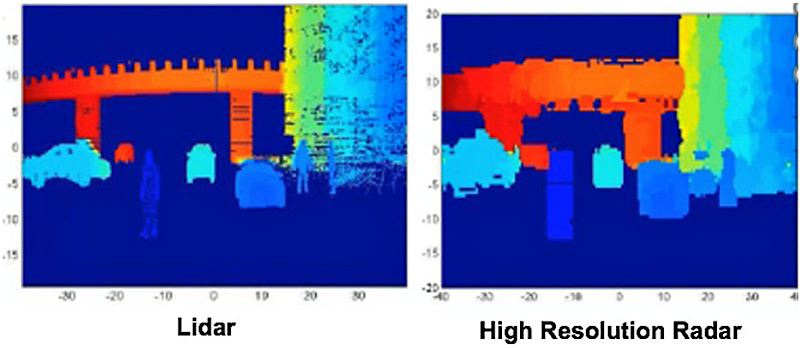
\includegraphics[width=\textwidth]{lidar-radar.png}
  \captionbelow[Vergleich Lidar und Radar Umgebungsscan]{Vergleich Lidar und Radar Umgebungsscan. (\cite{lidar-radar})}
  \label{lidar-radar}
\end{figure}

In den Fahrzeugen von Waymo, einem Tochterkonzern von Google's Mutterkonzern Alphabet, sind drei \acs{Lidar}-Scanner auf dem Dach der Fahrzeuge verbaut (siehe \ref{waymo-lidar}). Dazu gehören ein Kurzstrecken-\acs{Lidar} für den unmittelbaren Bereich um das Fahrzeug, ein Langstrecken-\acs{Lidar}, der auch aus mehreren hundert Metern Entfernung und voller Geschwindigkeit feine Signale, wie Handbewegungen, erkennen kann sowie einem hoch auflösenden \acs{Lidar}, welcher Millionen Laserimpulse pro Sekunde aussenden kann, um ein detailliertes Bild der Umwelt zu erzeugen. \vgl{waymo-lidar} In autonomen Fahrzeugen wird \acs{Lidar} hauptsächlich für zwei Aufgaben eingesetzt:
\begin{enumerate}
  \item{Erkennung und Bestimmung von Objekten um das Fahrzeug}
  \item{Präzise Positionsbestimmung innerhalb der Fahrspur}
\end{enumerate}
\vgl{Surden}

\begin{figure}\centering
  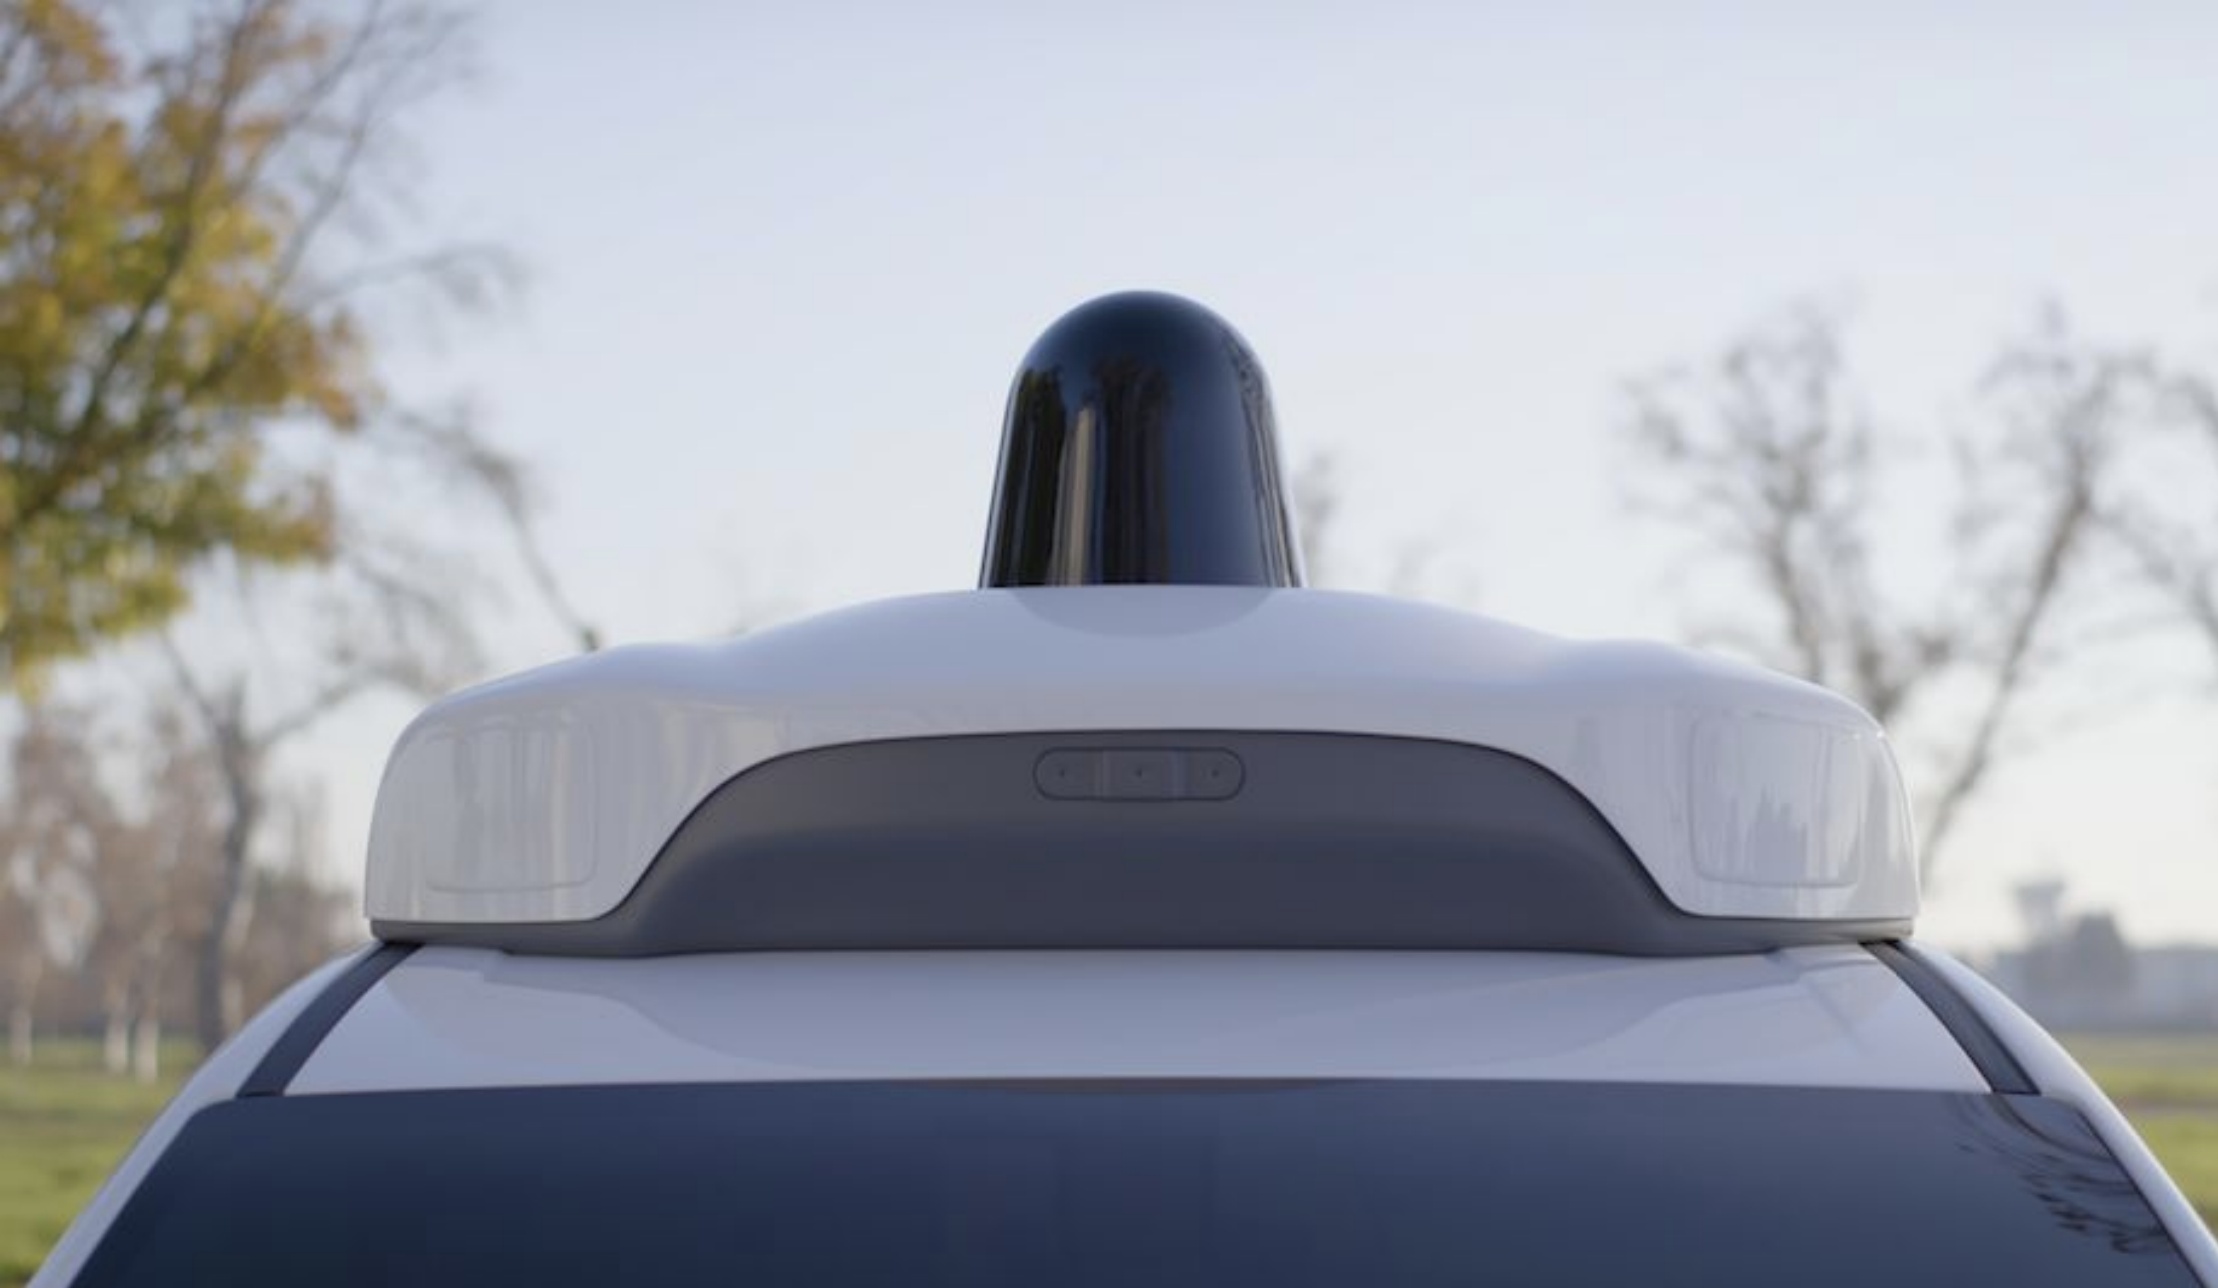
\includegraphics[width=\textwidth]{waymo-lidar.png}
  \captionbelow[Lidar-Scanner auf einem autonomen Fahrzeug von Waymo]{Lidar-Scanner auf einem autonomen Fahrzeug von Waymo. (\cite{waymo-lidar})}
  \label{waymo-lidar}
\end{figure}

\subsection{Partikel-Filter}

Eine Möglichkeit, um mittles \acs{Lidar}-Scannern die Position von Fahrzeugen bestimmen zu können, ist mittels Partikel-Filtern (auch Monte-Carlo-Lokalisierung). Hierfür wird auch eine annotierte digitale Karte (siehe \ref{maps}) benötigt, um vermessene Punkte mit den auf der Karte gespeicherten Objekten zu vergleichen.

\begin{enumerate}
  \item{Zuerst werden auf der Karte eine hohe Anzahl an sogenannten Partikeln verteilt. Jeder Partikel stellt eine mögliche Position des Fahrzeugs dar. Anfangs erhalten alle Partikel dieselbe Gewichtung (da die Position des Fahrzeugs gänzlich unbekannt ist), was bedeutet, dass alle Partikel die gleiche Wahrscheinlichkeit aufweisen, die korrekte Position darzustellen.}

  \item{Währrend sich das Fahrzeug bewegt, schickt es laufend Daten wie Geschwindigkeit und Winkel an den Fahrzeugcomputer. Jeder Partikel wird nun um dieselbe Distanz und in dieselbe Richtung wie das Fahrzeug bewegt, dieser Schritt nennt sich \textit{Prognose-Schritt}}.

  \item{Nun kommt der \textit{Vermessungsschritt}. Das Fahrzeug benutzt seine \acs{Lidar}-Scanner}, um die Distanzen zu den auf der Karte notierten markanten Punkten, zu vermessen. Jetzt werden für jeden Partikel ebenfalls die Distanzen zwischen dem Partikel und den markanten Punkten vermessen und anschließend mit den Vermessungen des Fahrzeugs verglichen. Partikel, die sich näher am Fahrzeug befinden, bekommen eine höhere Gewichtung zugewiesen.

  \item{Partikel, die unter eine gewisse Wahrscheinlichkeitsschwelle fallen, werden nun gelöscht und der Prozess ab Schritt 2 wird wiederholt.}
\end{enumerate}

Durch die ständige Wiederholung dieser Schritte ist es dem Fahrzeugcomputer möglich, dauerhaft die akurate Position des Fahrzeugs zu berechnen.
\vgl{particle-filter}

\subsection{BLMR-Methode}

Bei einer weiteren Möglichkeit, Fahrzeuge präzise zu lokalisieren, scannen \acs{Lidar}-Geräte Straßenmarkierungen, indem sie die Straßenoberfläche auf unterschiedliche Reflexionsvermögen (aufgrund weißer Markierungen) untersuchen und speichern die erfassten Daten in einer Datei namens \acs{BLMR} (\acl{BLMR}). In der \acs{BLMR} werden stets die Leit- und Randliniendaten der letzten \SI{240}{\meter} gespeichert, diese werden laufend mit den zuvor erstellten annotierten digitalen Karten (siehe \ref{maps}) abgeglichen, wodurch der Standort bestimmt werden kann. \vgl{self-localization}

Auch bei dieser Methode können sich die Sensoren automatisch an anderen markanten Punkten wie Straßenschildern, Ampelanlagen, Gebäuden oder Bäumen orientieren, sollten keine Straßenmarkierungen vorhanden sein. Wichtig ist nur, dass es sich bei den Objekten um Dinge handelt, deren Standort sich nicht ändert und die eindeutig für \acs{Lidar}-Scanner erkennbar sind.

\subsection*{Nachteile von Lidar}

Trotz der Vorteile wie der hohen Genauigkeit oder auch großen Reichweite haben auch \acs{Lidar}-Scanner Nachteile. Einer davon ist der Preis, besonders Geräte für große Distanzen sind teuer, da hierfür Laser mit einer Wellenlänge von \vgl{imu-def}\SI{1550}{\nano\meter} benötigt werden, um für Menschen nicht schädlich zu sein. Um solche Laserstrahlen wiederum empfangen zu können, sind Empfänger aus \ac{InGaAs} notwendig, da Siliziumempfänger, welche um ein Vielfaches günstiger als solche aus \ac{InGaAs} sind, keine Laserstrahlen mit \SI{1550}{\nano\meter} Wellenlänge erkennen können. \vgl{wired} Durch jahrelange Entwicklung und ständig steigenden Produktionszahlen hat es Waymo mittlerweile geschafft, die Kosten für einen \acs{Lidar}-Scanner von \$\,\num{75000} um 90\,\% auf \$\,\num{7500} zu reduzieren. \vgl{waymo-medium}

Ein weiterer Nachteil ist die Abhängigkeit von gutem Wetter. Schnee, Regen oder Nebel reflektieren das Licht, was zur Folge hat, dass das Fahrzeug fälschlicherweise Hindernisse erkennt, welche in Wirklichkeit nur Regentropfen oder Schneeflocken sind. Dieser Bereich unterliegt aktuell noch weiteren Forschungen, Ford hat jedoch schon einen Algorithmus entwickelt, der dieses Problem beheben soll. Dabei werden die empfangenen Laserstrahlen genau auf ihre Eigenschaften untersucht, etwa ob sich ein Objekt, von welchem der Laser reflektiert wird, zweimal an der selben Stelle befindet, was bei Regentropfen nicht der Fall ist.
\vgl{ford-qz}


\section{Positionsbestimmung ohne Lidar am Beispiel von Tesla}\label{section-2-3}

Anhand Teslas Fahrerassistenzsystem, dem sogenannten \enq{Autopilot}, lässt sich sehen, dass eine präzise Positionsbestimmung auch ohne \acs{Lidar}, sondern nur mit einer Kombination aus Ultraschallsensoren, Kameras und einem \acs{Radar}, möglich ist. Teslas aktuelle Autopilot 2.0 Hardware, mit der autonomes Fahren auf \ac{SAE}-Level 5 möglich sein soll, umfasst zwölf Ultraschallsensoren, acht Kameras sowie einen \acs{Radar} (siehe \ref{autopilot-hardware}).

\begin{figure}\centering
  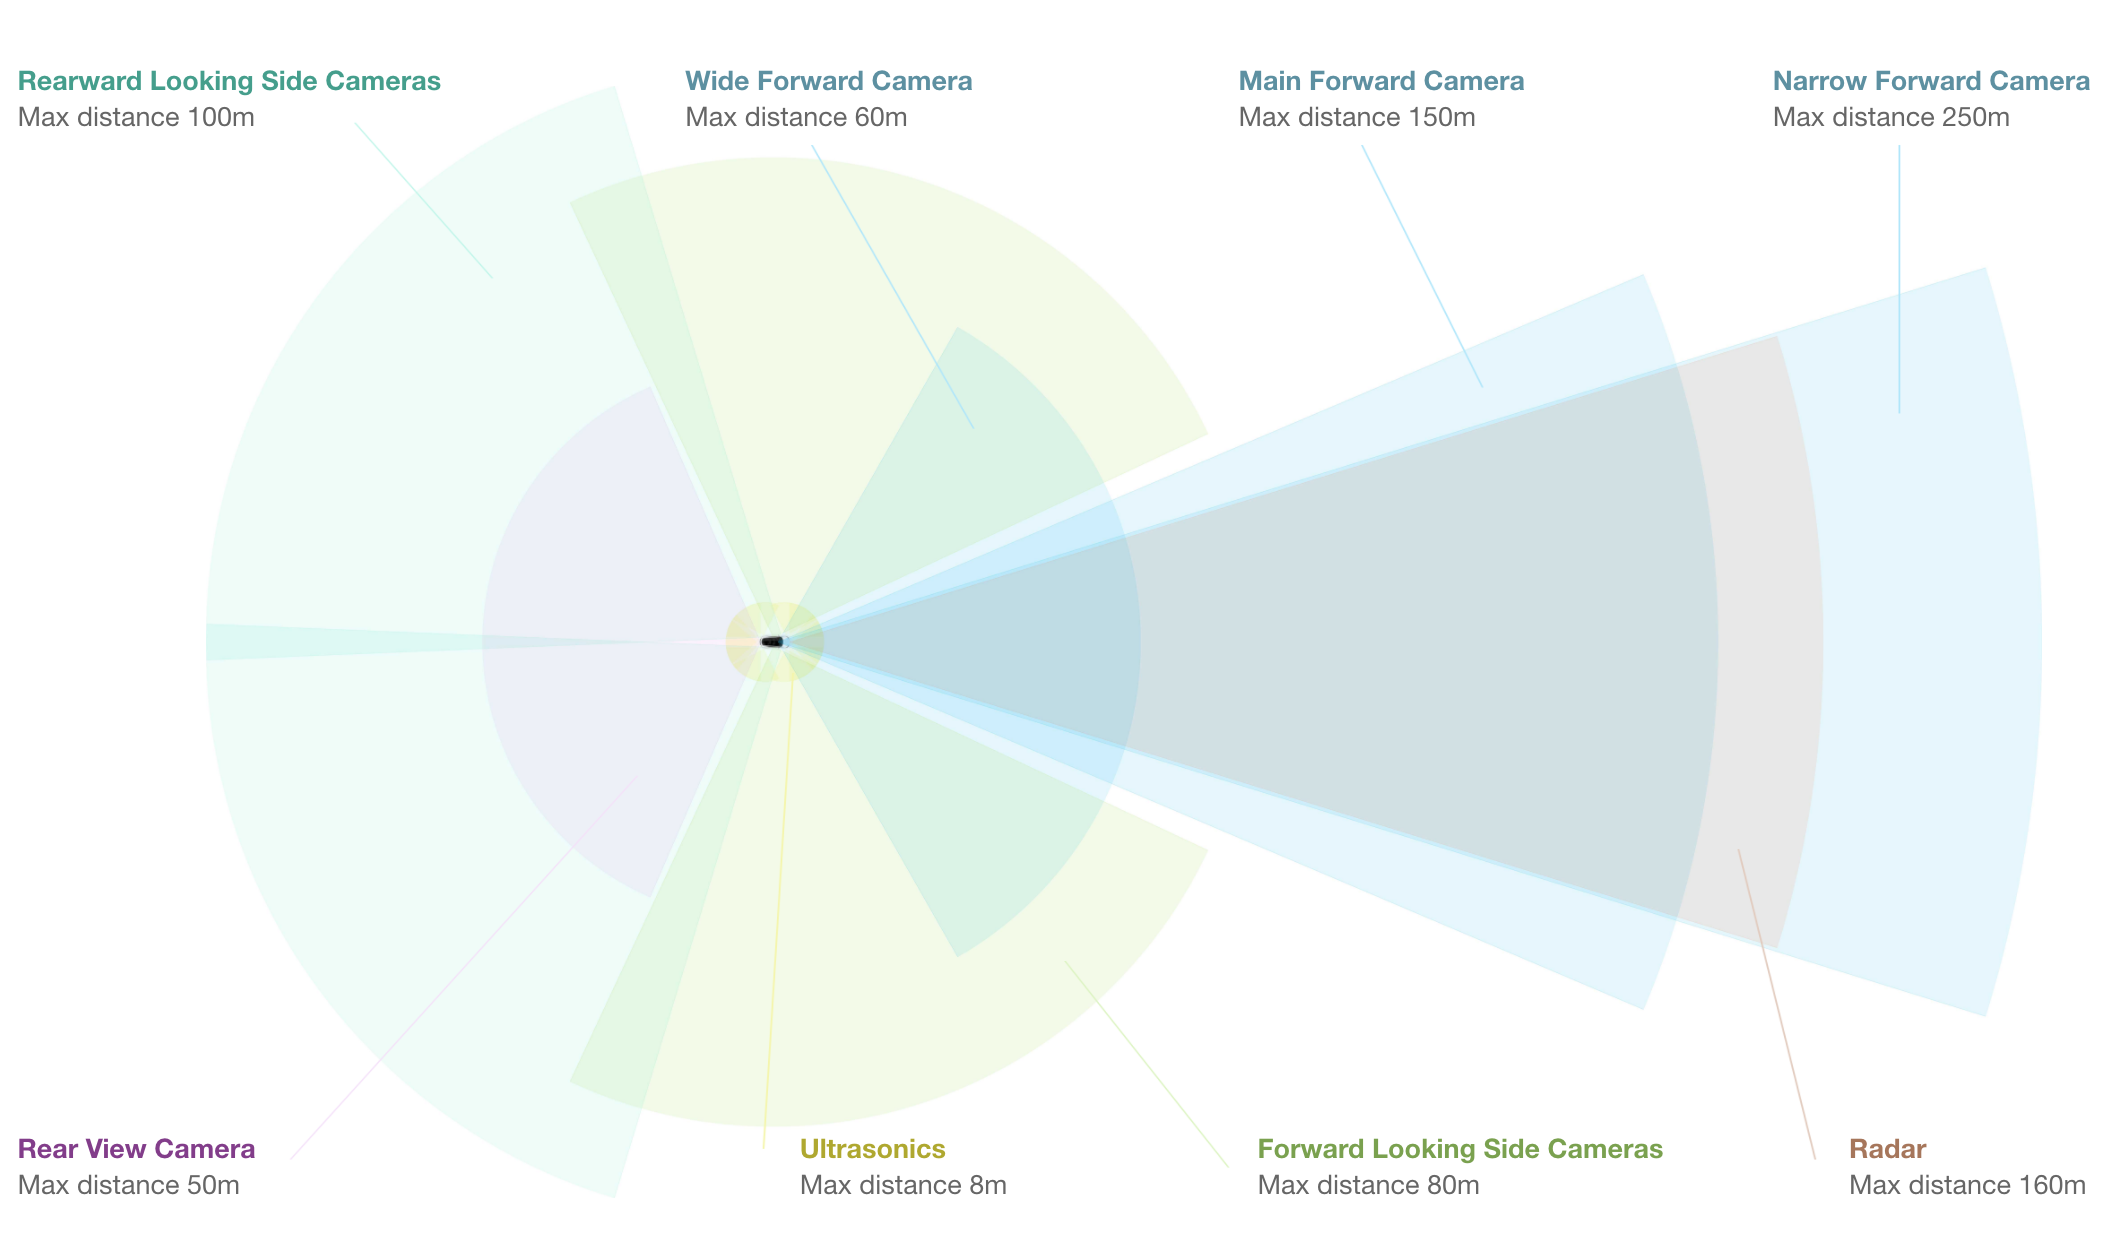
\includegraphics[width=\textwidth]{autopilot-hardware.png}
  \captionbelow[Tesla Autopilot 2.0 Hardware]{Tesla Autopilot 2.0 Hardware. (\cite{tesla-autopilot})}
  \label{autopilot-hardware}
\end{figure}

\noindent Elon Musk, CEO von Tesla, sagte in einem Konferanzanruf mit der Presse 2016: \zit{elon-musk}{We are confident that we can use the radar to look beyond the car in front of you by bouncing the radar signal off the road and around the car. \elp{}
So even if there’s something that was obscured directly both in vision and radar, we can use the bounce effect of the radar to look in front of that car and still brake.
It takes things to another level of safety.}

Mikrowellen eines \acs{Radar} ist es im Gegensatz zu Licht möglich, vom Boden zurückzuprallen. Dieser Umstand ermöglicht dem \acs{Radar}, unter einem vorherfahrenden Fahrzeug hindurch zu sehen und Gefahrensituationen frühzeitig zu erkennen, wodurch eventuell notwendige Notbremsmanöver rechtzeitig eingeleitet werden können. \vgl{ars-technica}

Außerdem verbaut Tesla in seinen Fahrzeugen keine \acs{Lidar}-Systeme, weil das Problem der Reflexion bei Regen, Nebel und Schneefall nicht besteht. Mikrowellen, wie die des \acs{Radar}, können diese Niederschläge durchdringen, wodurch keine fehlerhaften Erkennungen von Objekten entstehen, die gar nicht existieren. \vgl{ars-technica}
